\documentclass[oneside, 11pt]{article}

\usepackage[T1]{fontenc}
\usepackage[utf8]{inputenc}
\usepackage[dutch]{babel}

\usepackage{fouriernc}
\usepackage[detect-all, load-configurations=binary,
            separate-uncertainty=true, per-mode=symbol,
            retain-explicit-plus, range-phrase={ tot }]{siunitx}

\usepackage{setspace}
\setstretch{1.2}

\setlength{\parskip}{\smallskipamount}
\setlength{\parindent}{0pt}

\usepackage{geometry}
\geometry{marginparwidth=0.5cm, verbose, a4paper, tmargin=3cm, bmargin=3cm, lmargin=2cm, rmargin=2cm}

\usepackage{float}

\usepackage[fleqn]{amsmath}
\numberwithin{equation}{section}
\numberwithin{figure}{section}

\usepackage{graphicx}
\graphicspath{{Figures/}}
\usepackage{subfig}

\usepackage{tikz}
\usetikzlibrary{plotmarks}

\usepackage{fancyhdr}
\pagestyle{fancy}
\fancyhf{}
\rhead{\thepage}
\renewcommand{\footrulewidth}{0pt}
\renewcommand{\headrulewidth}{0pt}

\usepackage{relsize}
\usepackage{xspace}
\usepackage{url}

\newcommand{\figref}[1]{Figuur~\ref{#1}}

\newcommand{\hisparc}{\textsmaller{HiSPARC}\xspace}
\newcommand{\kascade}{\textsmaller{KASCADE}\xspace}
\newcommand{\sapphire}{\textsmaller{SAPPHiRE}\xspace}
\newcommand{\jsparc}{\textsmaller{jSparc}\xspace}
\newcommand{\hdf}{\textsmaller{HDF5}\xspace}
\newcommand{\aires}{\textsmaller{AIRES}\xspace}
\newcommand{\csv}{\textsmaller{CSV}\xspace}
\newcommand{\python}{\textsmaller{PYTHON}\xspace}
\newcommand{\corsika}{\textsmaller{CORSIKA}\xspace}
\newcommand{\labview}{\textsmaller{LabVIEW}\xspace}
\newcommand{\daq}{\textsmaller{DAQ}\xspace}
\newcommand{\adc}{\textsmaller{ADC}\xspace}
\newcommand{\adcs}{\textsmaller{ADC}s\xspace}
\newcommand{\Adcs}{A\textsmaller{DC}s\xspace}
\newcommand{\hi}{\textsc{h i}\xspace}
\newcommand{\hii}{\textsc{h ii}\xspace}
\newcommand{\mip}{\textsmaller{MIP}\xspace}
\newcommand{\hisparcii}{\textsmaller{HiSPARC II}\xspace}
\newcommand{\hisparciii}{\textsmaller{HiSPARC III}\xspace}
\newcommand{\pmt}{\textsmaller{PMT}\xspace}
\newcommand{\pmts}{\textsmaller{PMT}s\xspace}

\DeclareSIUnit{\electronvolt}{\ensuremath{\mathrm{e\!\!\:V}}}

\DeclareSIUnit{\unitsigma}{\ensuremath{\sigma}}
\DeclareSIUnit{\mip}{\textsmaller{MIP}}
\DeclareSIUnit{\adc}{\textsmaller{ADC}}

\DeclareSIUnit{\gauss}{G}
\DeclareSIUnit{\parsec}{pc}
\DeclareSIUnit{\year}{yr}



\title{Analyse met Coach}
\author{C.G.N. van Veen}
\docanalyse{4}{AC}
\version{1.0}

\begin{document}

\maketitle

\section{Inleiding}

Dit werkblad helpt leerlingen en docenten om data analyse van \hisparc met 
het software pakket Coach (6 of 7) te doen. Coach (6 of 7) is een software pakket wat leerlingen
en docenten in staat stelt om fysische grootheden te meten en analyses met deze 
data te doen. Coach is al op veel scholen beschikbaar en leerlingen kunnen hier
gemakkelijk mee aan de slag.
We gebruiken het onderdeel 'analyse' van Coach om ESD data van \hisparc te analyseren.
In dit document wordt stap voor stap uitgelegd hoe je deze data in kunt laden in 
Coach en kunt analyseren. Daarnaast wordt uitgelegd hoe je met deze data in Coach
grafieken kunt plotten en analyseren.

\section{Het ophalen van ESD data}

Ga naar de volgende website http://data.hisparc.nl en kies een station waar 
je data van wilt downloaden. Kies dan op de site waar je door te klikken terecht
bent gekomen de link aan de rechterkant: `Download event summary data'.
In info pakket kun je in het bestand `data retrieval' precies te zien hoe je 
nu de data als een excel bestand kunt downloaden.
Kies voor het gemak voor een dag data, dan is bestand nog redelijk klein.
Je krijgt een csv-bestand binnen waarin als eerste (de eerste 30 regels) beschreven staat wat je 
in elke kolom aan data vindt. In het csv-bestand vindt je onder andere, tijdstempel per event,
pulshoogte en pulsintegraal per detector, aantal deeltjes per detector en aankomsttijden van
de shower in de detector.

\section{Inlezen van de data in Coach.}

Het csv bestand gaan we inlezen in Coach. Open Coach, log in als docent en kies 'nieuwe activiteit' 
`meten'. Je hoeft geen paneel te kiezen.
Klik op het icoon tabel, zie \ref{fig:coach1}. Je kunt hier kiezen om een
nieuwe tabel aan te maken. Er verschijnt een werkvenster `tabel kiezen of maken'.
Kies in dit werkvenster `importeren'.


\begin{figure}
    \centering
    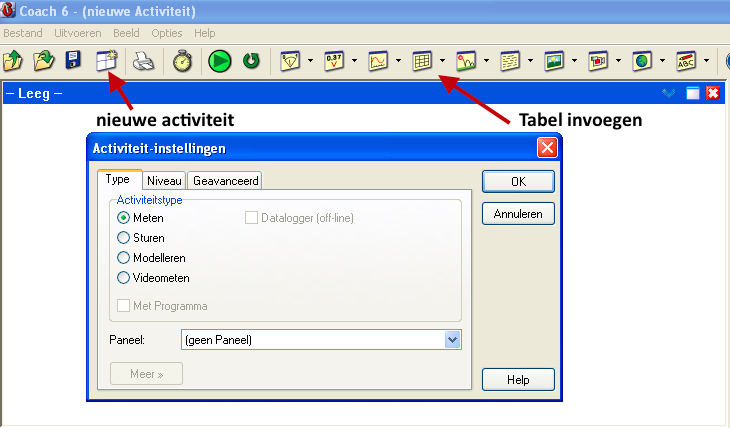
\includegraphics[scale=0.6]{coach1}
    \caption{screenshot van coach 6, open een nieuwe activiteit door op 
    het icoon linksboven te klikken (vier window icoon). Het icoon van tabel invoegen is
    aangegeven met de rechterpijl. Klik op dit icoon, er verschijnt dan een werkvenster.}
    \label{fig:coach1}
\end{figure}

\begin{figure}
    \centering
    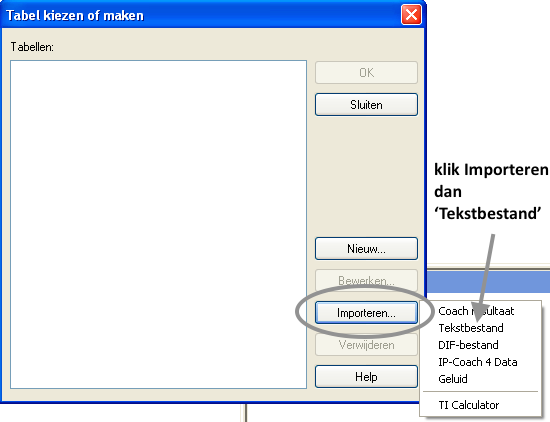
\includegraphics[scale=0.6]{coach2}
    \caption{Importeren van een csv-bestand met Coach. Kies tabel `importeren' en
    dan 'tekstbestand'.}
    \label{fig:coach2}
\end{figure}
   
\end{document}
